%%%%%%%%%%%%%%%%%%%%%%%%%%%%%%%%%%%%%%%%%
% Short Sectioned Assignment
% LaTeX Template
% Version 1.0 (5/5/12)
%
% This template has been downloaded from:
% http://www.LaTeXTemplates.com
%
% Original author:
% Frits Wenneker (http://www.howtotex.com)
%
% License:
% CC BY-NC-SA 3.0 (http://creativecommons.org/licenses/by-nc-sa/3.0/)
%
%%%%%%%%%%%%%%%%%%%%%%%%%%%%%%%%%%%%%%%%%

%----------------------------------------------------------------------------------------
%	PACKAGES AND OTHER DOCUMENT CONFIGURATIONS
%----------------------------------------------------------------------------------------

\documentclass[paper=a4, fontsize=11pt]{scrartcl} % A4 paper and 11pt font size

\usepackage[T1]{fontenc} % Use 8-bit encoding that has 256 glyphs
%\usepackage{fourier} % Use the Adobe Utopia font for the document - comment this line to return to the LaTeX default
\usepackage[english]{babel} % English language/hyphenation
\usepackage{amsmath,amsfonts,amsthm} % Math packages
\usepackage{mathtools} %More math! (For dscases)
\usepackage{hyperref} %HTML package
\usepackage{pgfplots} %Makes plots in LaTeX
\usepackage{tikz} %Also tikz?
\usepackage{bbm} %Blackboard bold 1
\usepgfplotslibrary{fillbetween}%Let's me fill between named plots
\usepackage{graphicx} %import pics
\graphicspath{ {Python_figs/} }
\DeclareGraphicsExtensions{.pdf,.png,.jpg}
\usepackage{sectsty} % Allows customizing section commands
\allsectionsfont{ \normalfont\scshape} % Make all sections the default font and small caps


\renewcommand{\thesubsection}{\alph{subsection}} %Make subsections start with letters

\usepackage{fancyhdr} % Custom headers and footers
\pagestyle{fancyplain} % Makes all pages in the document conform to the custom headers and footers
\fancyhead{} % No page header - if you want one, create it in the same way as the footers below
\fancyfoot[L]{} % Empty left footer
\fancyfoot[C]{} % Empty center footer
\fancyfoot[R]{\thepage} % Page numbering for right footer
\renewcommand{\headrulewidth}{0pt} % Remove header underlines
\renewcommand{\footrulewidth}{0pt} % Remove footer underlines
\setlength{\headheight}{13.6pt} % Customize the height of the header

\numberwithin{equation}{section} % Number equations within sections (i.e. 1.1, 1.2, 2.1, 2.2 instead of 1, 2, 3, 4)
\numberwithin{figure}{section} % Number figures within sections (i.e. 1.1, 1.2, 2.1, 2.2 instead of 1, 2, 3, 4)
\numberwithin{table}{section} % Number tables within sections (i.e. 1.1, 1.2, 2.1, 2.2 instead of 1, 2, 3, 4)

\setlength\parindent{0pt} % Removes all indentation from paragraphs - comment this line for an assignment with lots of text

%----------------------------------------------------------------------------------------
%	TITLE SECTION
%----------------------------------------------------------------------------------------

\newcommand{\horrule}[1]{\rule{\linewidth}{#1}} % Create horizontal rule command with 1 argument of height

\title{	Assignment 7}

\author{Benjamin Jakubowski} % Your name

\date{\normalsize\today} % Today's date or a custom date

\begin{document}

\maketitle % Print the title

%----------------------------------------------------------------------------------------
%	PROBLEM 1
%----------------------------------------------------------------------------------------

\section{Short questions}

\subsection{Fail to reject $\mathcal{H}_0$}

Failing to reject the null hypothesis does not mean that it is probably true. First and foremost (from a frequentist perspective), this statement is meaningless- the null hypothesis is either true or it is false. Moreover, failing to reject the null hypothesis may merely indicate we have an underpowered test (i.e. the probability of rejecting the null hypothesis given it is false is low). For example, consider repeatedly flipping a coin to test $\mathcal{H}_0: p = 0.5$ (where $p$ is the probability of heads). If the true probability of heads is $0.501$, with any reasonable sample size $n$ our test will be grossly underpowered and we will fail to reject $\mathcal{H}_0$ (even though it is false).

\subsection{Interpreting the p-value}

We cannot interpret the p-value as the probability the null hypothesis is true. Again (as previously mentioned) from a frequentist perspective this statement is meaningless since the null hypothesis is either true or it is false. Instead, we can intuitively understand the p-value as the probability of our test statistic being as or more 'extreme' than the observed value under $\mathcal{H}_0$.

\subsection{Size and power during exploratory analysis}

During the exploratory phase of analysis, we would rather use a test with a large size and large power. Since we want to identify possible effects that show up in the data, we want to minimize the rate of type II errors (which, in the context of the question, would mean missing real effects). While this will mean we make more type I errors (incorrectly reject the null when in reality there is no effect), this is not a primary concern given we are only exploring the data and can assume we will reduce the occurrence of type I errors through subsequent analyses. 

\subsection{Size and power in subsequent analyses}

If we have identified a possible effect and want to make sure it is not just due to random noise, we should use a test with a small size and small power. Since we want to minimize the possible of making a type I error (i.e. rejecting the null hypothesis even though the observed effect is due only to random noise), we should prioritize having small size over having large power.

\subsection{Problem of applying Bonferroni's method}

When testing a large number of hypotheses, the problem with applying Bonferroni's method is that it is too conservative. Bonferroni's method is based on the union bound, which (in this context) implies:
\begin{align*}
\textrm{P(Type I error) } &= \textrm{P}(\cup_{i=1}^n \textrm{Type I error for test } i) \\
   &= \left[\sum_{i=1}^{n} \textrm{P}(\textrm{Type I error for test } i)\right] - k \\
   &=n \cdot \frac{\alpha}{n} - k \\
   &\leq \alpha
\end{align*}
where $k\geq0$ is a correction for the probability of an intersection of (some subset of) the events "Type I error for test $i$", $i \in \{1, 2, ..., n \}$. Importantly, $k$ is a non-decreasing function of the number of  $n$ (the number of hypothesis tests) since adding an additional hypotheses can only increase, not decrease, the probability of an intersection. Thus, as $n$ grows large the Bonferroni-adjusted $\alpha_{Bonferroni} = \frac{\alpha}{n}$ becomes unnecessarily conservative, and as a result the Type II error rate will increase.

%----------------------------------------------------------------------------------------
%	PROBLEM 2
%----------------------------------------------------------------------------------------

\section{Cars}
\subsection{Hypothesis test based on $\textrm{max}_{1 \leq i \leq n} T_i$}

First, recall the company wants to make sure the cars won't have any problems for at least a year on average. Since the time until a car breaks down for the first time (call it $T$) is well modeled as an exponential random variable, we want:
\[E[T] = \frac{1}{\lambda} \geq 1 \implies 1 \geq \lambda\]

Thus, our hypotheses are:
\begin{align*}
\mathcal{H}_0&: \lambda > 1 \\
\mathcal{H}_1&: \lambda \leq 1
\end{align*}

Again, our test statistic is $X(\textbf{T}) = \textrm{max}_{1 \leq i \leq n} T_i$. Our rejection region is 
\[ \mathcal{R} := \{x | x \geq \eta\} \]
where $\eta$ is selected based on the desired size of the test.

\subsection{Power function for test}

The power function of our test is
\begin{align*}
\beta(\lambda) &= P_{\lambda}(X(\textbf{T}) \in \mathcal{R}) \\
   &= P_{\lambda}(X(\textbf{T}) \geq \eta) \\
   &= P_{\lambda}( \textrm{max}_{1 \leq i \leq n} T_i \geq \eta) \\
   &= 1 - P_{\lambda}(\cap_{i=1}^{n}T_i < \eta) \\
   &= 1 - \prod_{i=1}^{n} P_{\lambda}(T_i < \eta) \qquad{} \textrm{ (by IID)} \\
   &= 1 - \prod_{i=1}^{n} \left( 1 - e^{- \lambda \eta} \right)\\
   &= 1 - \left( 1 - e^{- \lambda \eta} \right)^n
\end{align*}


\subsection{Plots of the power function for different $n, \eta$}

Several plots for different values of $n$ and $\eta$ are shown on the next page. Holding $n$ constant, as $\eta$ increases power decreases for all $\lambda$. On the other hand, holding $\eta$ constant, as $n$ increases power increases for all $\lambda$. 
\begin{center}
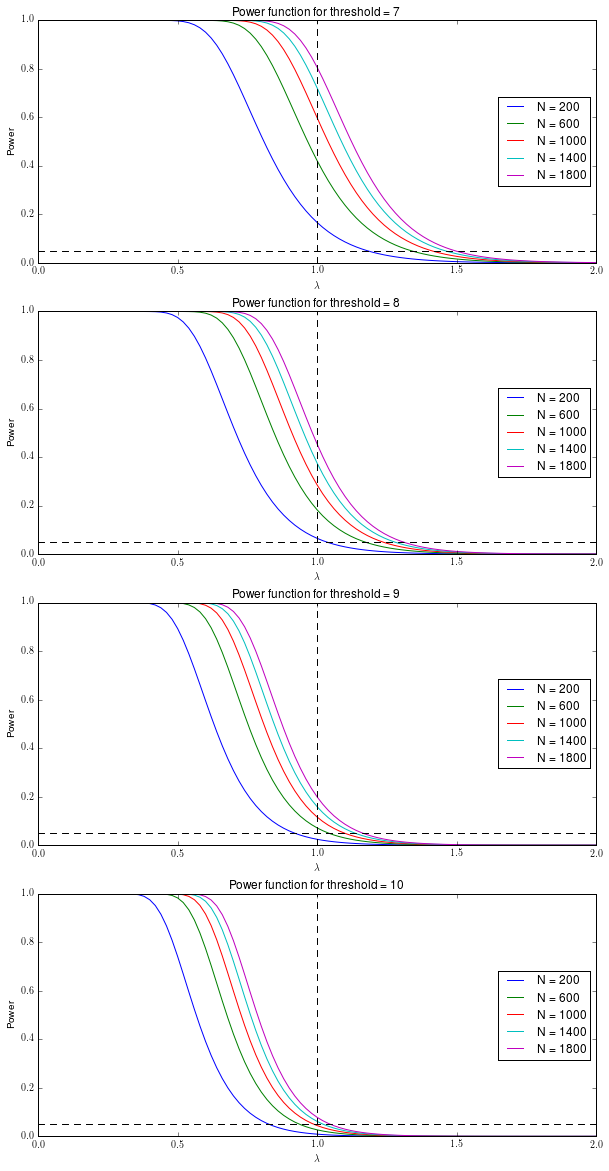
\includegraphics[scale=0.5]{Q2c_fig} 
\end{center}

%----------------------------------------------------------------------------------------
%	PROBLEM 3
%----------------------------------------------------------------------------------------

\section{Sign test}

\subsection{Null hypothesis for sign test}

First recall our friends conjecture is that in general the left ear of most people is longer than the right ear.
Now let $L_i$ be the length of person $i$'s left ear and $R_i$ be the length of person $i$'s right ear. Then our test statistic is:
\[T(\textbf{X}) = \sum_{i=1}^{n} \mathbbm{1}_{L_i > R_i} \]

Our hypotheses are:
\begin{align*}
\mathcal{H}_0&: \textrm{ There is no difference in the length of most peoples left and right ear.} \\
\mathcal{H}_1&:  \textrm{ In general, the left ear of most people is longer than the right ear.}
\end{align*}

\subsection{Size of the test in terms of $n$}

Under our null hypothesis, the probability that a person's left ear is longer than their right ear is 1/2, so the distribution of our test statistic is binomial with parameter $n$ (in this case, $n$ = 10) and $p = 0.5$. Thus, our rejection region is of the form
\[ \mathcal{R} := \{ t | t \geq \eta\}\]
with $0 \leq \eta \leq n$ given based on the desired size. Then
\begin{align*}
\alpha &= P(T_0 \geq \eta)\\
   &= \frac{1}{2^n} \sum_{k = \eta}^n {n \choose k}
\end{align*}

\subsection{Significance level of our data}

In our data, in 7 of the 10 observations the left ear is longer than the right ear. Thus, our p-value is:
\begin{align*}
p &= P(T_0 \geq 7)\\
   &=  \frac{1}{2^n} \sum_{k = 7}^n {n \choose k}\\
   &=  \frac{1}{2^{10}} \sum_{k = 7}^{10} {10 \choose k}\\
   &= 1 - 0.828 = .172
\end{align*}
With such a large p-value, we clearly fail to reject $\mathcal{H}_0$.

%----------------------------------------------------------------------------------------
%	PROBLEM 4
%----------------------------------------------------------------------------------------

\section{Permutation test for the median}

\subsection{P-values for the difference of the sample median}

Using a permutation test for the median, we have
\begin{center}
   \begin{tabular} { | c | c |} \hline 
      \textbf{Trial} & \textbf{P-value} \\ \hline
      Trial 1 & 0.00178 \\ \hline
      Trial 2 & 0.00199 \\ \hline
      Trial 3 & 0.00163 \\ \hline
   \end{tabular}
\end{center}

In contrast, using the permutation test for the mean, we have 
\begin{center}
   \begin{tabular} { | c | c |} \hline 
      \textbf{Trial} & \textbf{P-value} \\ \hline
      Trial 1 & 0.00113 \\ \hline
      Trial 2 & 0.00112 \\ \hline
      Trial 3 & 0.00106 \\ \hline
   \end{tabular}
\end{center}

\subsection{Interpreting this observed difference in p-values for mean/median}

Since there are a number of outliers (3 men with extremely high cholesterol levels), the mean registers a more significant difference between men and women than the mean. This is because the mean more sensitive to these extreme observations. On the other hand, the median is more robust to outliers, and as such the observed difference in median cholesterol levels is less significant. \\
As a side note, we can can conduct a simple thought experiment to confirm our intuition about the sensitivity of the mean and median to outliers- imagine replacing the extreme observations (three men with cholesterol levels around 400) with absurd observations (three men with cholesterol levels around 100000). This would clearly bias the mean, but it would have no effect on the median.

%----------------------------------------------------------------------------------------
%	PROBLEM 5
%----------------------------------------------------------------------------------------

\section{Most published research findings are false}

In his 2005 essay, \emph{Why Most Published Research Findings are False}, John Ioannidis constructs and analyzes confusion matrices using several parameters:
\begin{itemize}
\item $R$: the ratio of "true relationship" to "no relationship" (field-level parameter)
\item $\alpha$: the size of the statistical test used to claim the presence of a relationship (study-level parameter)
\item $\beta$: the power of the statistical test used to claim the presence of a relationship (study-level parameter)
\item $c$: the number of relationships being probed in the field (field-level parameter)
\item $u$: Proportion reflecting inflation of "true relationship" claims due to bias (a study-level parameter)
\item $n$: Number of studies addressing a research question (a field-level parameter)
\end{itemize}
Based on this parameterization, he is able to show that most "true relationship" claims are false (i.e. the positive predictive value PPV of a published positive finding is low). More over, certain fields have particularly low PPVs, including fields using high-throughput methods (for example '-omics' methods in the biological sciences) to probe large numbers of potential relationships (i.e. large $c$) in the absence of compelling prior evidence of relationships (i.e. low $R$). Interestingly, his essay suggests the "Data Science" project is relatively ill-advised (see Table 4, which suggests "Discovery-oriented exploratory research with massive testing" has a PPV on the order of 0.0010). Instead, studies with high PPVs are relatively conventional "adequately powered RCT with little bias and 1:1 pre-study odds".

%----------------------------------------------------------------------------------------
\end{document}